%TODO
%	- run cluster and descriptors tests
%	- find out what's wrong with sift detector
%	- run detector tests
%	- prepare strategy pattern class diagram and describe it
%	- write conclusions
%	- describe libraries
%	- write abstracts
%	- go through introduction
%
%
%

\documentclass[12pt]{report}
\usepackage[utf8]{inputenc}
\usepackage[T1]{fontenc}
\usepackage[a4paper, top=2.5cm, bottom=2.5cm, left=2.5cm, right=2.5cm]{geometry}
\usepackage{cite}
\usepackage{graphicx}
\usepackage{color}
\usepackage[font=footnotesize]{caption}
\usepackage{amsmath}
\usepackage[hidelinks]{hyperref}
\usepackage{paralist}
\usepackage{tocbibind}
%\usepackage[nottoc,notlof,notlot]{tocbibind}

%\renewcommand{\chaptername}{}
%\renewcommand{\thechapter}{}

\linespread{1.5}

\newcommand{\superscript}[1]{\ensuremath{^{\textrm{#1}}}}
\newcommand{\subscript}[1]{\ensuremath{_{\textrm{#1}}}}
\newcommand\rednote[1]{\textcolor{red}{#1}}

\makeatletter
% Redefine the \chapter* header macro to remove vertical space
\def\@makeschapterhead#1{%
  %\vspace*{50\p@}% Remove the vertical space
  {\parindent \z@ \raggedright
    \normalfont
    \interlinepenalty\@M
    \Huge \bfseries  #1\par\nobreak
    \vskip 20\p@
  }}
\makeatother

\bibliographystyle{abbrv}
\begin{document}



\pagestyle{empty}
\color{white} . \color{black}
\vspace{0.2cm}

\begin{center}
\begin{Huge}Warsaw University of Technology
\end{Huge}
\end{center}

\begin{center}
\begin{LARGE}Faculty of Mechatronics

\vspace{0.5cm}
Institute of Automation and Robotics
\vspace{1.0cm}
\end{LARGE}
\end{center}
\begin{center}
\includegraphics[width=5cm,angle=0]{figs/logopw}\end{center} 

\vspace{0.5cm}

\begin{center}
\begin{LARGE}\textbf{Adam Kosiorek}\end{LARGE}
\end{center}

\vspace{0.5cm}

\begin{center}
\begin{Huge}\textbf{3D Object Classification based on RGBD images}
\vspace{0.5cm}
\end{Huge}
\end{center}

\vspace{0.5cm}

\begin{center}
\begin{Large}bachelor thesis written under supervision of\end{Large}

\vspace{0.2cm}

\begin{Large}prof. dr. hab. Barbara Siemiątkowska\end{Large}
\end{center}

\vspace{1.8cm}

\begin{center}
\begin{Large}Warsaw 2014\end{Large}
\end{center}


%    \vspace*{1\baselineskip}
    \begin{tabular}{p{5cm} p{10cm}}
    \begin{minipage}{5cm}
    \center
    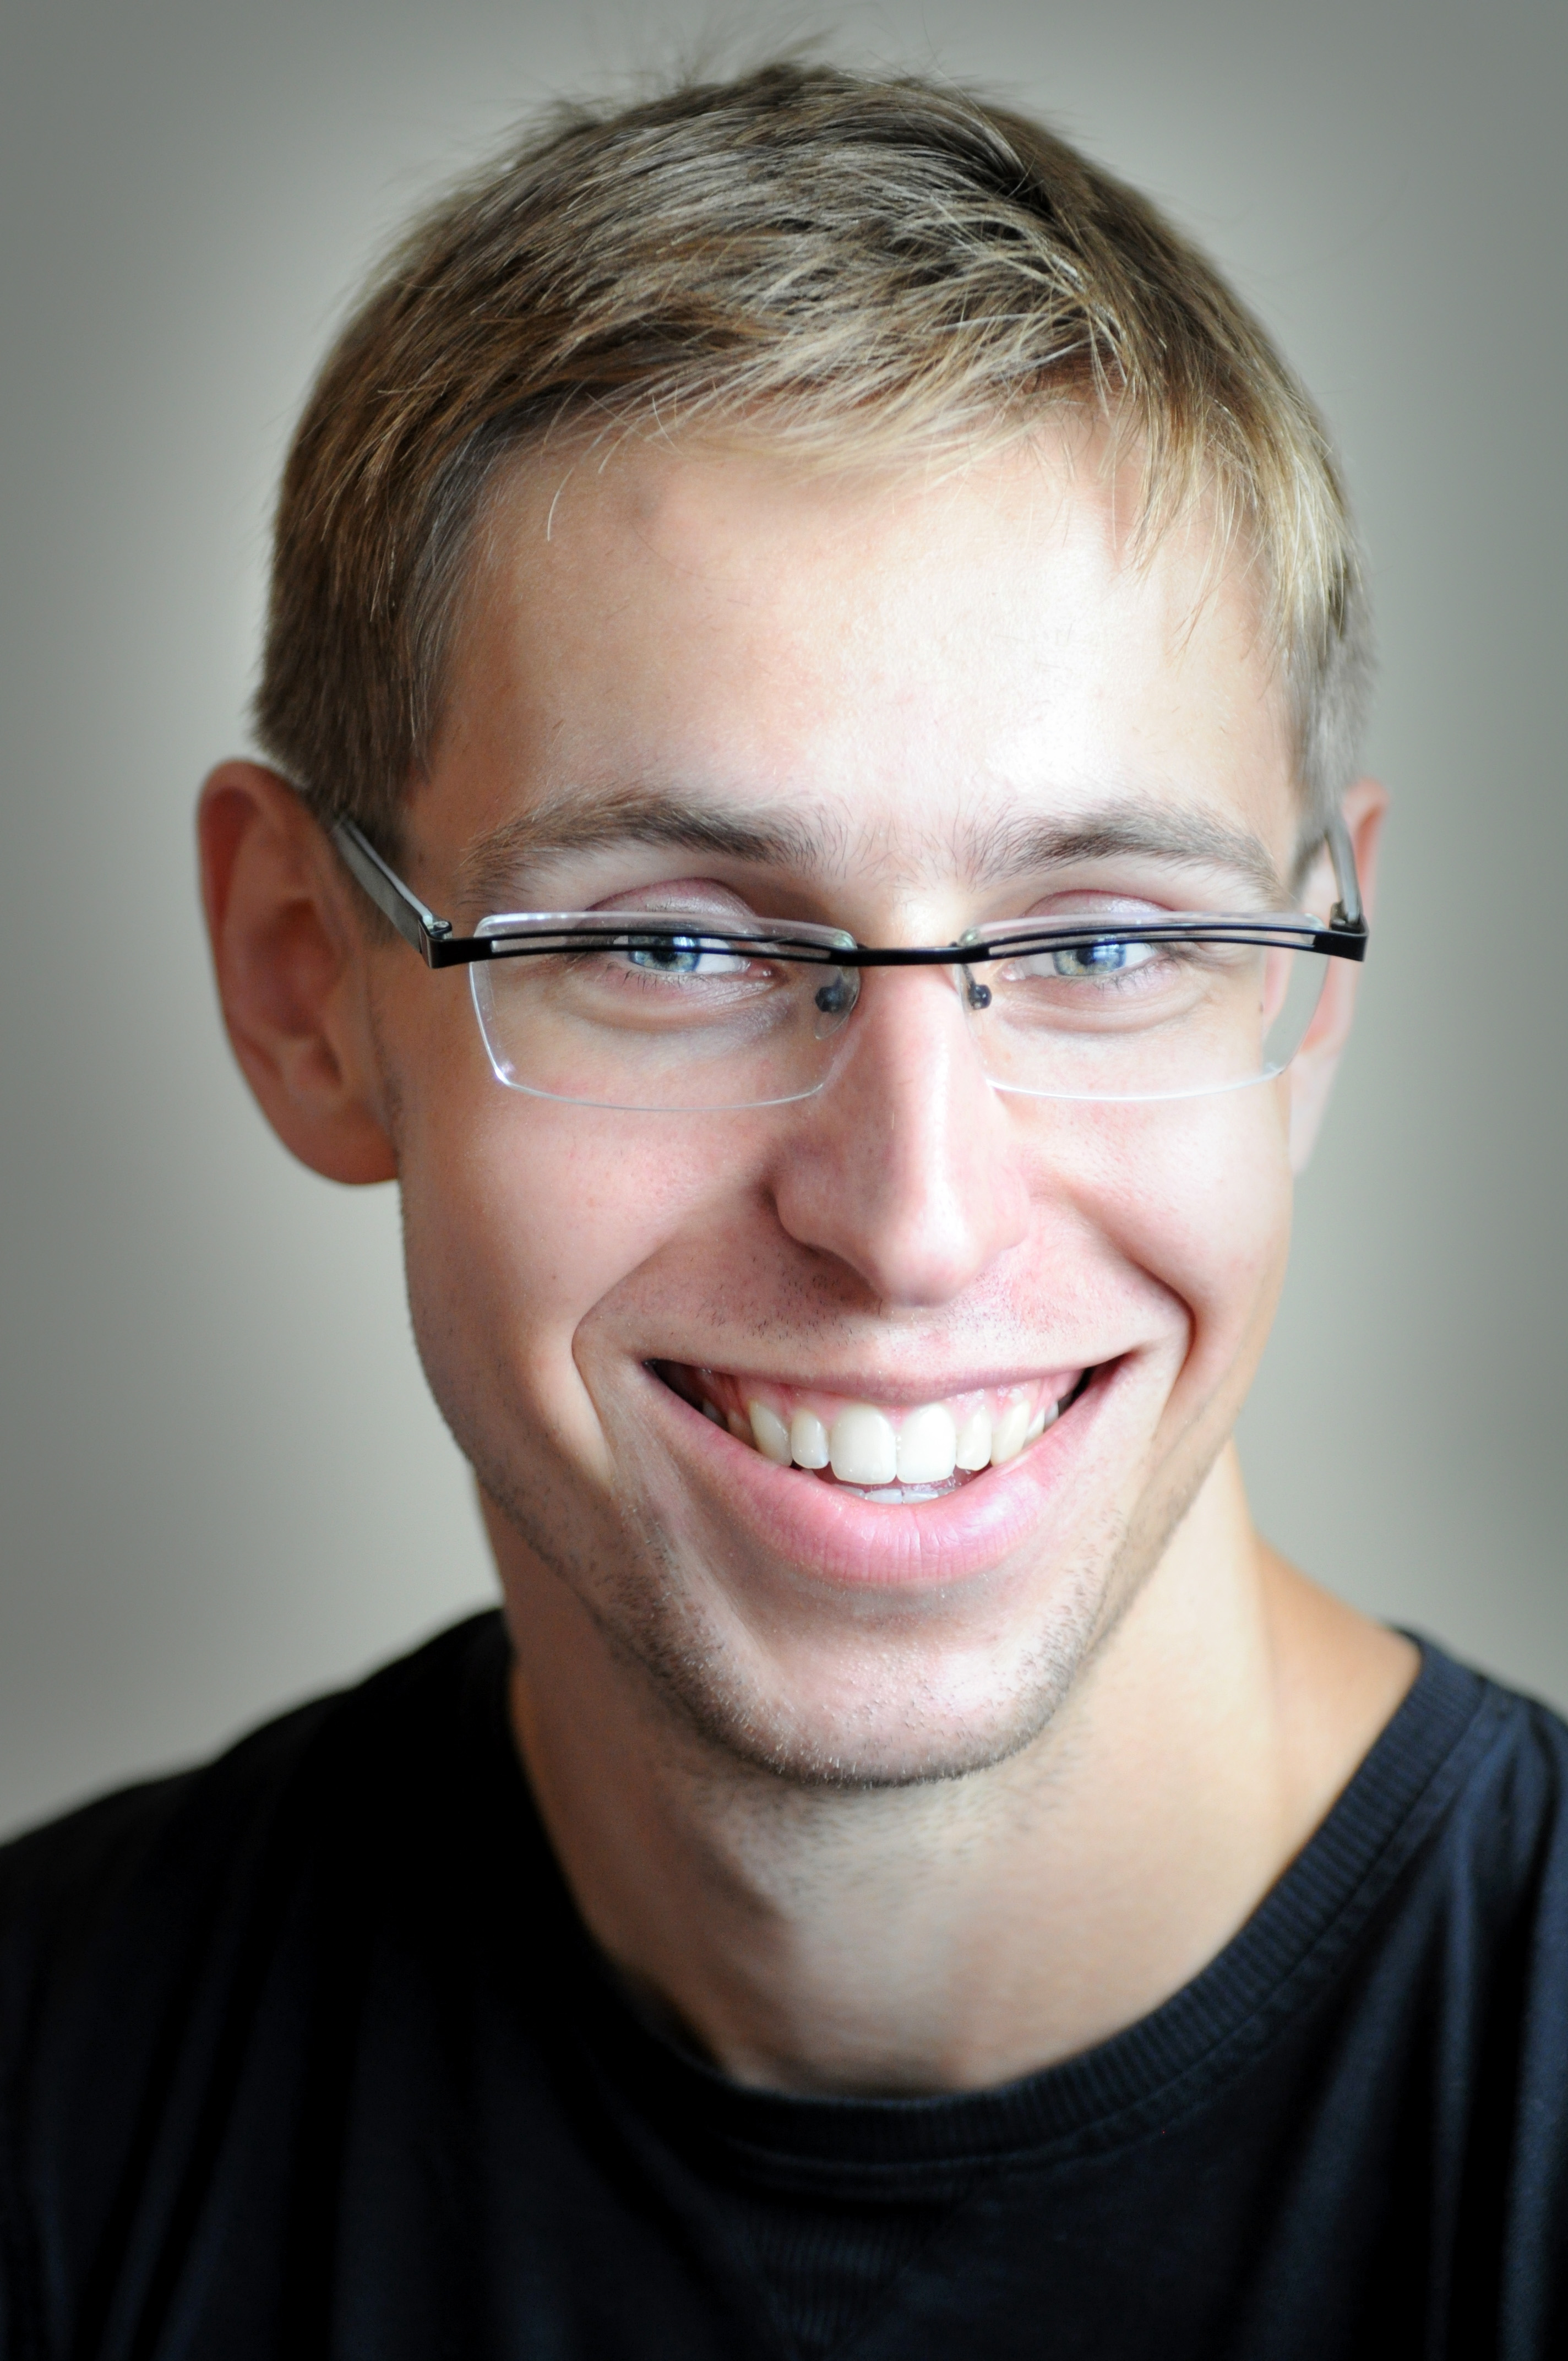
\includegraphics[width=4.5cm]{figs/ja}
    \end{minipage}
    &
    \begin{minipage}{12cm}
\par\noindent\vspace{1\baselineskip}
    \begin{flushleft}
    \par\noindent\vspace{1\baselineskip}
    \begin{tabular}[h]{l l}
    {\normalsize\it Degree:} & Automatic Control Engineering and Robotics
    \end{tabular}
    \par\noindent\vspace{1\baselineskip}
    \begin{tabular}[h]{l l}
    {\normalsize\it Major:} & Robotics
    \end{tabular}
    \par\noindent\vspace{1\baselineskip}
    \begin{tabular}[h]{l l}
    {\normalsize\it Birth date:} & {\normalsize 28 February 1991}
    \end{tabular}
    \par\noindent\vspace{1\baselineskip}
    \begin{tabular}[h]{l l}
    {\normalsize\it Study starting date:} & {\normalsize 1 October 2010 r.}
    \end{tabular}
    \par\noindent\vspace{1\baselineskip}
    \end{flushleft}
    \end{minipage}
    \end{tabular}
    \vspace*{1\baselineskip}
    \begin{center}
	{\large\bfseries Biography}\par\bigskip
    \end{center}
	
	I was born on 28 February 1991 in Olsztyn, Poland. I attended 5\superscript{th} Secondary School by the name of ``The Common Europe'' in Olsztyn. I started a Bachelor of Engineering degree on the Faculty of Mechatronics of Warsaw University of Technology on 1 October 2010. I did an internship in Faurecia R\&D S.A. in 2012. In 2013 I started working in IBM Poland Sp. z o.o. where I stayed for 6 months. Then I started working full-time in Samsung R\&D Centre Poland.
	
    \par
    \vspace{3\baselineskip}
    \hfill\parbox{15em}{{\small\dotfill}\\[-.3ex]
    \centerline{\footnotesize signature}}\par
    \vspace{3\baselineskip}

\pagestyle{plain}

\begin{center}
\begin{LARGE}\textbf{Abstract}\end{LARGE}
\end{center}

\vspace{1.0cm}

Properties of special generalized functions and short-range selectors which are indispensable in the Shina Tan description of interacting Fermi systems [Annals of Physics 323, 2952 (2008)] are analyzed in details. Also all details of the proof of the Shina Tan energy theorem and properties of the contact are presented. The manuscript should be interesting for researchers who want to understand all elements of the Shina Tan extraordinary work.

\tableofcontents


\section{Introduction}

	introduction
\chapter{Design and Implementation}
%\addcontentsline{toc}{chapter}{Design}

\section{Software Functionality and Architecture}
	
	We have decided to call our project ``Tagger3D''.  Since the purpose is to classify (or tag) point clouds, the name seems suitable. An optimal combination of algorithms for a bag of words pipeline is task and data specific. To find a combo of routines that yields superior performance we have to evaluate numerous algorithms. The process can be simplified; We are going to design an application that can be easily configured and extended. It should be possible to configure and choose an algorithm at run-time. Moreover, it should enable real time classification if it is to be used in any real setting.
	
	\subsection{Required functionality}	
	There are three major functions that have to be supported by the programme:
	\begin{enumerate}
	 \item train --- performs training
	 \item test --- evaluates the previously trained classifier
	 \item infer --- predicts a category of a single object
	\end{enumerate}
	
	Before any of them can be implemented, we have to identify common features. Inference and testing is very similar. The only difference is that the latter should process a whole testing dataset and compute statistics. The inference and training processes looks as follows:
	
	\begin{tabular}{p{0.5\textwidth}p{0.5\textwidth}}
		Inference:
		\begin{enumerate}
			\item RGBD image reading and preprocessing
			\item Point cloud construction
			\item Salient region identification
			\item Feature Extraction
			\item Vector Quantization
			\item Classification
		\end{enumerate} 
		&
		Training:
		\begin{enumerate}
		\item RGBD image reading and preprocessing
		\item Point cloud construction
		\item Salient region identification
		\item Feature Extraction
		\item Codebook Construction
		\item Vector Quantization
		\item Classificator training
		\end{enumerate} \\
	\end{tabular}
	
	The only differences is that training stage requires codebook construction and classifier training, whereas inference uses the classifier for prediction. If we compare training to testing it is clear that they both deal with large amounts of data. Inference is not that data-intensive and can be carried out for a single image. In order to simplify training we have decided to split the training and testing phases into several sub-routines. Such treatment let us change settings of an algorithm without the need to retrain the stages that lay before considered algorithm in the pipeline (\emph{e.g.} there is no need to extract features once more only because we have changed the dictionary size). The final application has the following operational modes, accessible from the command line:
	
	\begin{enumerate}
		\item Feature Extraction
		\item Codebook Generation
		\item Classifier Training
		\item Classifier Evaluation
		\item Inference
	\end{enumerate}
	
	In order to ensure that the application is configurable and easily extensible we used singleton and strategy design patterns and resorted to the Boost's program\_options package for configuration file parsing.
	
		\subsubsection{Input/Output operations}	
		This work is extremely data dependent. Every operation requires external data. Both training and testing a classifier consumes hundreds of images. Datasets used in this projects have different and incompatible formats. Not only an object responsible for run-time input/output operations is needed, but also a set of scripts for data preprocessing. Additionally, some serialisation method have to be supplied. The training of the classifier is far too computationally expensive to be computed every time the application starts. Once the classifier is trained, all the models should be stored for further usage. A way of saving and loading codebook and svm model is required. 
		
		\subsubsection{Configuration}		
		Every algorithm used in this work have several configuration parameters. If the parameters were to be compiled with the code, every change would require a rebuild of parts of the application. A run-time configuration functionality is essential. 
		
		\subsubsection{Interchangeability of algorithms}		
		Multitude of available algorithms makes it time consuming and computationally expensive to evaluate every available option. It should be possible to build the programme with a number of algorithms suitable for performing the same task and decide which one should be used at run-time.
		
	\subsection{Architecture}
	
	\begin{figure}[ht]
	\centering
	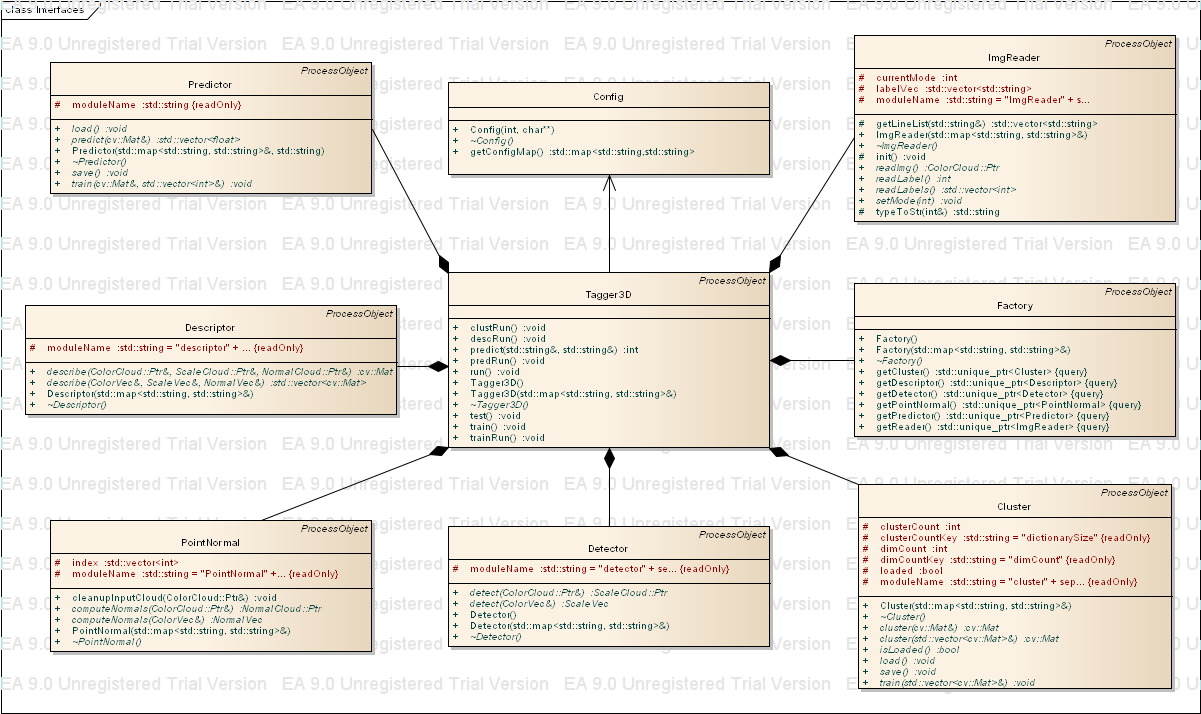
\includegraphics[width=1.0\textwidth]{figs/class}
	\caption{Tagger3D class diagram}
	\label{fig:class_diagram}
	\end{figure}
	
	C++ is one of the most efficient languages on the market. It is perfect for Object Oriented Programming (OOP) --- a paradigm that makes writing modular, flexible and extensible software easier. The excellent meta-programming tools provided by the language help to minimise the length of the hand-written code. Among OOP's best practices is to use design patterns - a set of well-known, documented and tested methods of solving certain architectural problems. Using design patterns leads to cleaner code which is easier to maintain and reuse. 
	
	\subsubsection{Configurability}
	The programme is configurable through a text file of a standard *.ini format. It should be formatted as follows:\\ \ \\
	 param1 = 2\\
	 param2 = aha\\
	 {[section]}\\
	 param3 = no\\
	
	On top of the file there is a global section. Parameters can be accessed by their names. We can define sections but putting a section's name in brackets. the param3 can be accessed as ``section.param3''. An object ``Config'' was created for the purpose of configuration file parsing. It uses the Boost.program\_options module. Returned associative array of (parameter, value) pairs contains all parameters from a configuration file. We use a convention that if any object has to be configured by the configuration map it has to accept this map in it's constructor.
	
	\subsubsection{Strategy Design Pattern}
	
	\begin{figure}[ht]
	\centering
	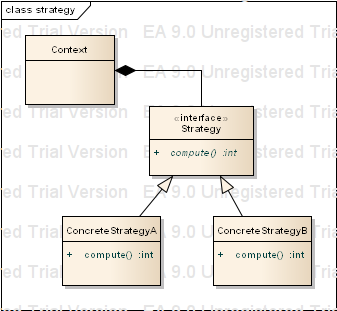
\includegraphics[width=0.5\textwidth]{figs/strategy}
	\caption{Strategy pattern}
	\label{fig:strategy}
	\end{figure}
	
	Design patterns were for the very first time by Gamma \emph{et al} in 1993 \cite{gamma1993design}. They are best practices that should be used to solve recurring problems in software design. One of the patterns is the strategy pattern. It enables implementation of multiple algorithms to handle one task. Then, a specific algorithm can be selected at run-time. It is the exact problem encountered here. It is stated that an interface should be defined for each task and multiple classes encapsulating different algorithms for handling the task should realise the interface. One modification has been done: Algorithms have often some common operations, thus an idea of an interface (a class without any implemented methods) was dropped in favour of an abstract class with some methods implemented. 
	
	The strategy pattern was used for every processing step of the pipeline so as to make it extensible. This property can be enhanced further by using a pattern of abstract factory. The idea was dropped in this case, however. The project is relatively small and the bulk of an abstract factory is beyond reason.
	
	Six parts of the pipeline are a subject of strategy pattern. The interfaces representing them are: ImgReader, PointNormal, Detector, Descriptor, Cluster, Predictor. Each of them contains pure virtual computation methods --- 'read` in case of the ImgReader or 'predict' in case of the Predictor. Additionally, they have some common methods defined --- I/O methods in Cluster or batch processing methods (such that take a vector of elements instead of a single element as an input) for the Detector and the Descriptor. Every pure virtual class have its specialisations. For instance there is the PFHDescriptor class with a Point Feature Histogram descriptor or a KMeansCluster employing kMeans clustering algorithm. The Factory class chooses specialisations of the algorithms at run-time, depending on the configuration parameters.
	
\section{Implementation}

	The complete program consists of more than 5600 lines of code in C++ and additional several hundreds of code in data preprocessing scripts.
	
	\subsection{Data preprocessing scripts}
		\begin{description}
			\item[imgListPrep.py] A script in python we have written for the purpose of listing hundreds of images (colour images and depth maps) and their corresponding labels in text files. These files are later used for batch processing such as training, but also for further data preprocessing.
			\item[b3doPrep] A short C++ programme used for object extraction from the B3DO dataset. It uses TinyXML, a lightweight C++ library for XML processing. It reads lists of files(depth maps, colour images and image annotations stored in the XML format) and iterates over them. Each iteration consists of loading an image, extracting labels and locations of bounding boxes from the XML, extracting the regions of interests and saving them at a new location.
			\item[divImgsByCats.py] Another short python script. Used mainly for splitting all the extracted objects into separate folders, one for every category.
			\item[pcdPrep] One more short C++ application. It was created for the reason of handling the Tokyo dataset. The dataset comes in a rather difficult-to-manage form. This application processes the raw files and saves them as point clouds in a PointCloud Library's PCD format.	 
			\item[grid.py and easy.py] These python scripts are an integral part of the libsvm library. Usually distributed as executables with the library, they help to perform corssvalidation and avoid overfitting. We have modified both scripts significantly in order to tune their performance on the very specific hardware describe in the Experiments section.
		\end{description}
		
		While the data prepared by pcdPrep is readily available for usage by the main programme the case with the B3DO dataset is quite different. The colour images and depth maps still have to be converted to point clouds because any further processing can be undertaken. That is because if the application were to work on-line with a Microsoft Kinect plugged in, it would have to handle the raw data from Kinect, which comes in a form of two images.

	\subsection{Conversion of colour images and depth maps into point clouds}
	
		The colour data and the depth data come from different cameras. The colour data come from 640 x 320 RGB camera, while the depth data come from active 320 x 240 infrared sensor. Only after registration the depth data is interpolated to match the colour data in resolution. Even after that operation, however, individual points from both images does not match exactly. That might introduce noise into the point cloud. We have not solved this issue and so that would be an area for further improvement. It did, however, focused our attention on another problem. If the two images do not fit perfectly it might be the case that one of the cameras have registered some points that had been invisible for the other one. Precisely, if there are any points in the colour image that the depth camera have not captured their depth would be meaningless. The Kinect's firmware does, in fact, address this issue. The depth value of every such point is set to NaN or Not a Number values. Before proceeding to the next stage we filter out all points, whose depth value has been set to NaN;
		
		Another problem is that only the Z coordinate is given explicitly in the depth map. The XY coordinates have to be inferred from the Z coordinate and the point's location relative to the sensor. We assumed that the sensor's position should correspond to the middle of the image or the the pixel at (320, 240). The Kinect specification says that the horizontal and vertical fields of view are respectively $57^{\circ}$ and $43^{\circ}$. We can compute the coordinates as: \\
		
		\begin{centering}
			$factorH = tg (\frac{57}{2}) * \frac{\pi}{180}$\\
			$factorV = tg (\frac{43}{2}) * \frac{\pi}{180}$\\
			$X = depth * factorH * (pixelX / 320)$\\
			$Y = depth * factorV * (pixelX / 240)$\\
			$Z = depth$\\
		\end{centering}
		
	\subsection{Input/Output Objects}
	
		As stated in the input/output section above, the application is very data dependent. Therefore, some objects for input/output operations were designed and implemented. The whole public API is delivered by the IoUtils class. It's methods allow reading and writing of text files, binary files of different formats, vectors of elements, vectors of vectors of elements and OpenCV's Mat objects. Elements that can be worked with are all C/C++ primitive types, all user defined types with defined std::string toString() method and OpenCV's Mat objects. In order to enhance performance, the IoUtils statically uses an object of type VectorIO for any vector input/output operation. The VectorIO is a template class parametrized by a type that is to be read into or written from a vector to a file on a hard drive. The VectorIO class uses a default implementation for all C/C++ primitive type and has template specialisations for the following types: std::vector, std::string, cv::Mat, any user defined object with a public std::string toString() method. Moreover, both IoUtils and VectorIO uses custom type trait classes that provide file extensions, size of types in bytes or processing algorithms for different data types.
		
		





\section{Experiments}
\subsection{Detectors}
\subsection{Descriptors}
\subsection{Codebook}
\subsection{B3DO}
\subsection{tokyo}

\listoffigures
\listoftables
	
\bibliography{eng}

\appendix
\chapter{Source code}
	The source code of the main programme as well as all the scripts and a sample configuration file are included on an attached CD.
\end{document}

